\section {Desarrollo}

\subsection{Preparación del \textit{corpus} y preprocesamiento}

Optamos por subir el \textit{dataset} a Google Drive, una decisión motivada por la necesidad de contar con una 
ubicación centralizada y accesible desde entornos de computación en la nube, como Google Colab. Esta elección 
facilitó la integración del \textit{dataset} en el \textit{pipeline} de trabajo, al permitir su descarga automática 
mediante \texttt{gdown}, una herramienta que posibilita la descarga directa desde Google Drive al entorno de ejecución.

Los datos, estructurados en archivos CSV (\texttt{train.csv} y \texttt{test.csv}), contenían metadatos demográficos 
y temporales que enriquecieron el contexto semántico de los textos, como el país de origen, la edad del usuario y 
el sentimiento del \textit{tweet}. Este último resultó fundamental para la tarea de clasificación, aunque los demás 
no pudieron ser aprovechados en este trabajo.

El proceso de extracción empleó \texttt{ThreadPoolExecutor} para descomprimir los archivos en paralelo mediante 
hilos de forma optimizada. Se eliminó el directorio \texttt{\_\_MACOSX} con el fin de garantizar la integridad del 
\textit{dataset}, eliminando residuos generados por sistemas operativos ajenos al entorno experimental, en este caso,
macOS. 

Durante la carga de los archivos, se utilizó la codificación \texttt{ISO-8859-1}, ya que con \texttt{UTF-8} se 
presentaban caracteres no reconocidos, lo que impedía una correcta lectura de los datos.

Para el tratamiento lingüístico, se implementó un proceso de normalización del texto que consistió en la eliminación de 
caracteres especiales mediante expresiones regulares, conversión a minúsculas para homogeneizar el léxico y tokenización 
utilizando la clase \texttt{Tokenizer} de \texttt{Keras}

Se utilizó la técnica de \textit{skip-grams} debido a su capacidad para capturar relaciones contextuales entre palabras. Este enfoque permitió generar 
pares de palabras formados por una palabra objetivo y su contexto, logrando un equilibrio entre la detección de patrones y la distribución del 
vocabulario. Hemos implementado una función propia de \textit{skip-grams}, ya que la versión de \texttt{Keras} se encuentra deprecada y no reflejaba 
fielmente el contexto real de cada oración, dado que introducía índices aleatorios dentro del tamaño del vocabulario al pasarle una única oración 
del \textit{dataset}.

\begin{figure}[H]
    \centering
    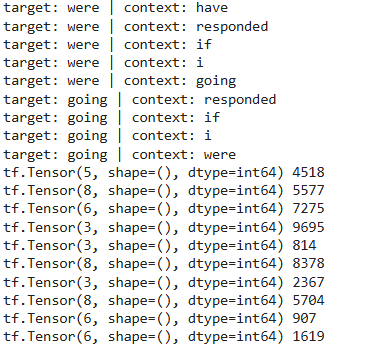
\includegraphics[height = 4.2cm]{ImagenesLatex/random_skip.png}{}
    \caption{Ejemplo del uso de \textit{skip-grams} de \texttt{Keras} que muestra índices aleatorios}
    \label{fig:random_skip}
\end{figure}

\vspace{5px}

\subsection{Arquitectura del modelo}

